%************************************************
\chapter{Hypothetical Knowledge}
\label{chapter:hypothetical_knowledge}
%************************************************

\section{Hypotheses}

I have previously described grounded factual knowledge that has an
unquestionable basis in symbolic perceptions.  Now, I will describe
how hypothetical causal models are abstracted from this factual
knowledge in order to create counterfactual knowledge, which keeps
this factual references so that it can be debugged when it is wrong.

\section{Hypothesis Space}

\cite{mitchell:1997} presents a general formalism for learning
hypotheses from sets of ground truth examples.  He describes a
function approximation approach to the discrimination problem of
predicting a binary value given a set of binary features.  In order to
keep the model of learning as general as possible, Mitchell introduces
the concept of a \emph{hypothesis space}.  Given a language for
describing hypotheses, the hypothesis space includes all possible
expressions in this language.  The hypothesis language can be
arbitrarily general, but in order to demonstrate my thesis about
reflective thinking, I make the simplifying assumption that this
language is simply based on the logical ``and'' expression.  This is
called the \emph{conjunctive hypothesis space}.  The conjunctive
hypothesis space consists of all logical conjunctions of the input
features.
{\mbox{\autoref{figure:example_hypothesis}}}.
\begin{figure}
\center
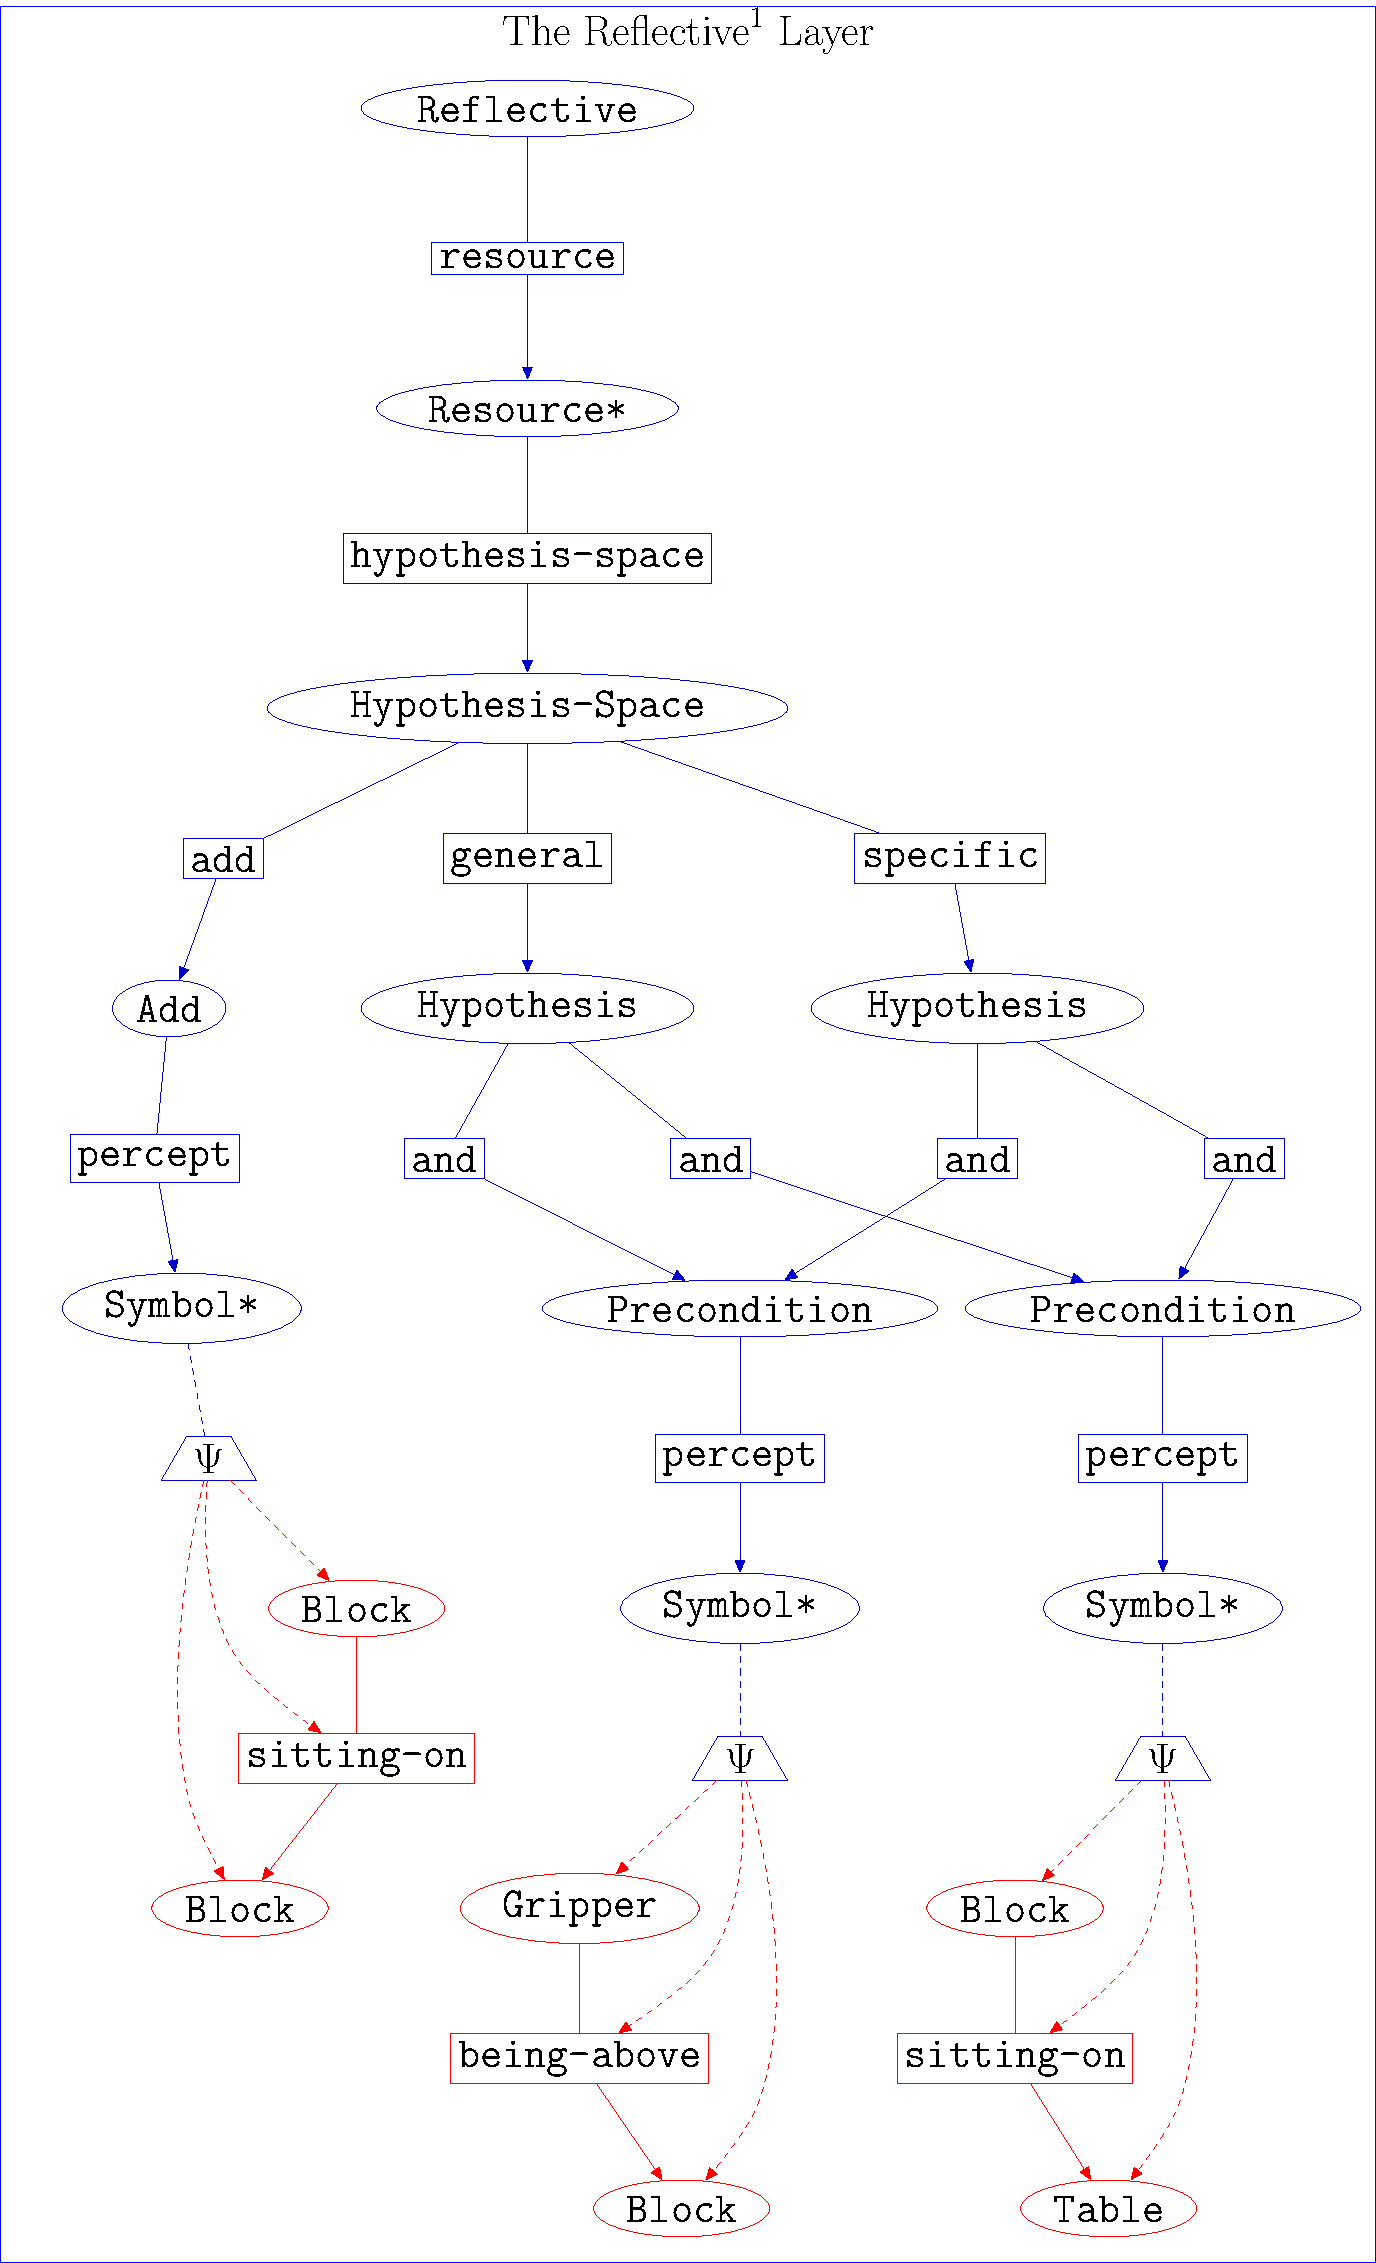
\includegraphics[width=8cm]{gfx/example_hypothesis}
\caption[An example of a hypothesis.]{An example of a hypothesis.}
\label{figure:example_hypothesis}
\end{figure}

\section{The General-to-Specific Ordering of Hypotheses}

\begin{definition}
\emph{Let $h_j$ and $h_k$ be Boolean-valued functions defined over
  $X$. Then $h_j$ is more-general-than-or-equal-to $h_k$ (written
  $h_j\ \geq_g\ h_k$) if and only if
\begin{equation*}
\forall_{x \in X}, [(h_k(x) = 1) \rightarrow (h_j(x) = 1)]
\end{equation*}
}\end{definition}

Depending on the choice of hypothesis language, it is not always
trivial to determine whether one hypothesis is more general than
another.  All non-redundant hypotheses in the conjunctive hypothesis
space of four input variables is shown as ordered in a generalization
lattice in
{\mbox{\autoref{figure:example_conjunctive_hypothesis_space}}}.
\begin{figure}
\center
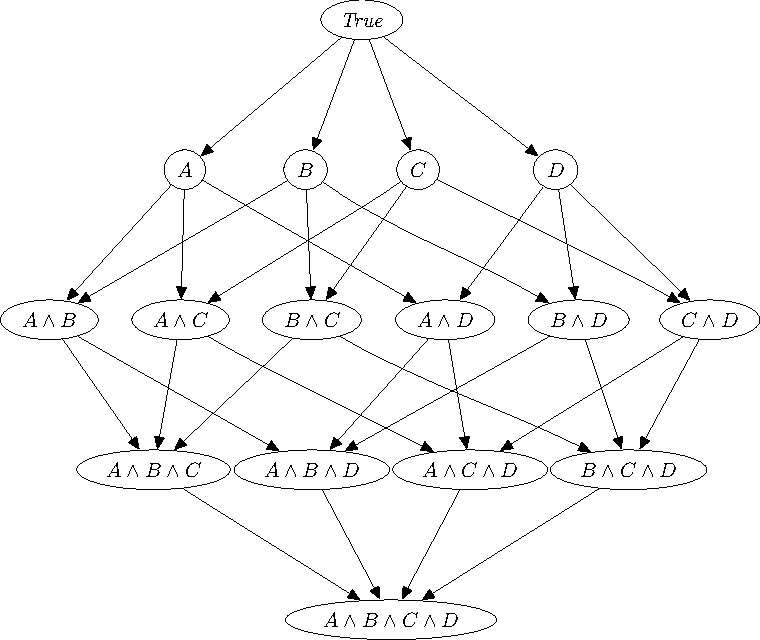
\includegraphics[width=8cm]{gfx/example_conjunctive_hypothesis_space}
\caption[An example of a conjunctive hypothesis space.]{An example of
  a conjunctive hypothesis space of four logical variables, $A$, $B$,
  $C$, and $D$.  All possible conjunctive hypotheses represented as
  nodes in a lattice with general-to-specific orderings represented by
  edges.}
\label{figure:example_conjunctive_hypothesis_space}
\end{figure}

\section{Concept Version Spaces}

Given a general-to-specific ordering of the entire hypothesis space,
Mitchell describes an efficient representation of all hypotheses that
match a given set of input examples, which he calls a \emph{version
  space}.  The implementation uses this very efficient version space
representation to keep track of all hypotheses in the conjunctive
hypothesis space that are consistent with factual knowledge.
%{\mbox{\autoref{figure:example_conjunctive_version_space}}} shows an
%example of a hypothesis version space.
%\begin{figure}
%\center
%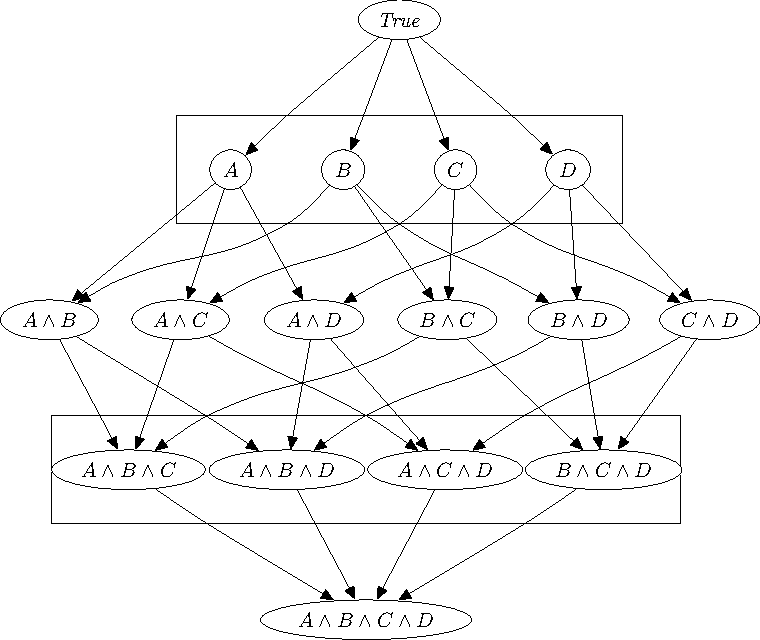
\includegraphics[width=8cm]{gfx/example_conjunctive_version_space}
%\caption[An example of a conjunctive hypothesis version space.]{An
%  example of a conjunctive hypothesis version space.}
%\label{figure:example_conjunctive_hypothesis_space}
%\end{figure}

%\begin{equation}
%{n\choose k} = \frac{n!}{k!(n-k)!}
%\end{equation}

\section{Hypothesizing Transframes from Preconditions}

In the model, planning is based on predicting the hypothetical effects
of resource actions.  In order to predict counterfactual
simultaneities, which can fill future slots of counterfactual
transitions, each historical resource activation transframe is
considered as input to a hypothesis version space concept learning
algorithm.

Equations\ \ref{equation:define_resource_precondition_symbols}
and\ \ref{equation:define_resource_transframe_symbols} define the
precondition symbols, $a^*_E$, that can be used to hypothetically
predict the transframe symbols, $a^*_D$, for the general execution of
the action resource, $a^*$.
\begin{align}
\label{equation:define_resource_precondition_symbols}
  a^*_X &= \bigcup_{\epsilon \in a^*.\text{\tt{activation}}} [\text{pre}^{+}(\epsilon) \cup \text{pre}^{-}(\epsilon)] \\
\label{equation:define_resource_transframe_symbols}
  a^*_D &= \bigcup_{\epsilon \in a^*.\text{\tt{activation}}} [\Delta^{+}(\epsilon) \cup \Delta^{-}(\epsilon)]
\end{align}
%Equation\ \ref{equation:define_know_event_transframe_delta} defines
%the factual ground knowledge of a transframe change, $\delta$, given
%the action resource factual event, $a^*_\epsilon$.
%\begin{equation}
%\label{equation:define_know_event_transframe_delta}
%   \text{added}(\delta | a^*_\epsilon) = \left\{\begin{array}{ll}
%                                                 \text{\emph{True}}  & \text{~if $\delta \in \Delta^{+}(a^*_\epsilon)$} \\
%                                                 \text{\emph{False}} & \text{~if $\delta \in \Delta^{-}(a^*_\epsilon)$} \\
%                                                 \text{undefined}    & \text{~otherwise} \\
%                                               \end{array}\right.
%\end{equation}

\section{leftovers...}

\section{Causal Knowledge}

Now that a separate temporal sequence for each reflective layer has
been defined, this factual grounded knowledge can be abstracted into
hypothetical causal models that are useful for planning toward goals
in a counterfactual future.



{\mbox{\autoref{figure:example_causal_knowledge}}} shows an example of
causal knowledge.
\begin{figure}
\center
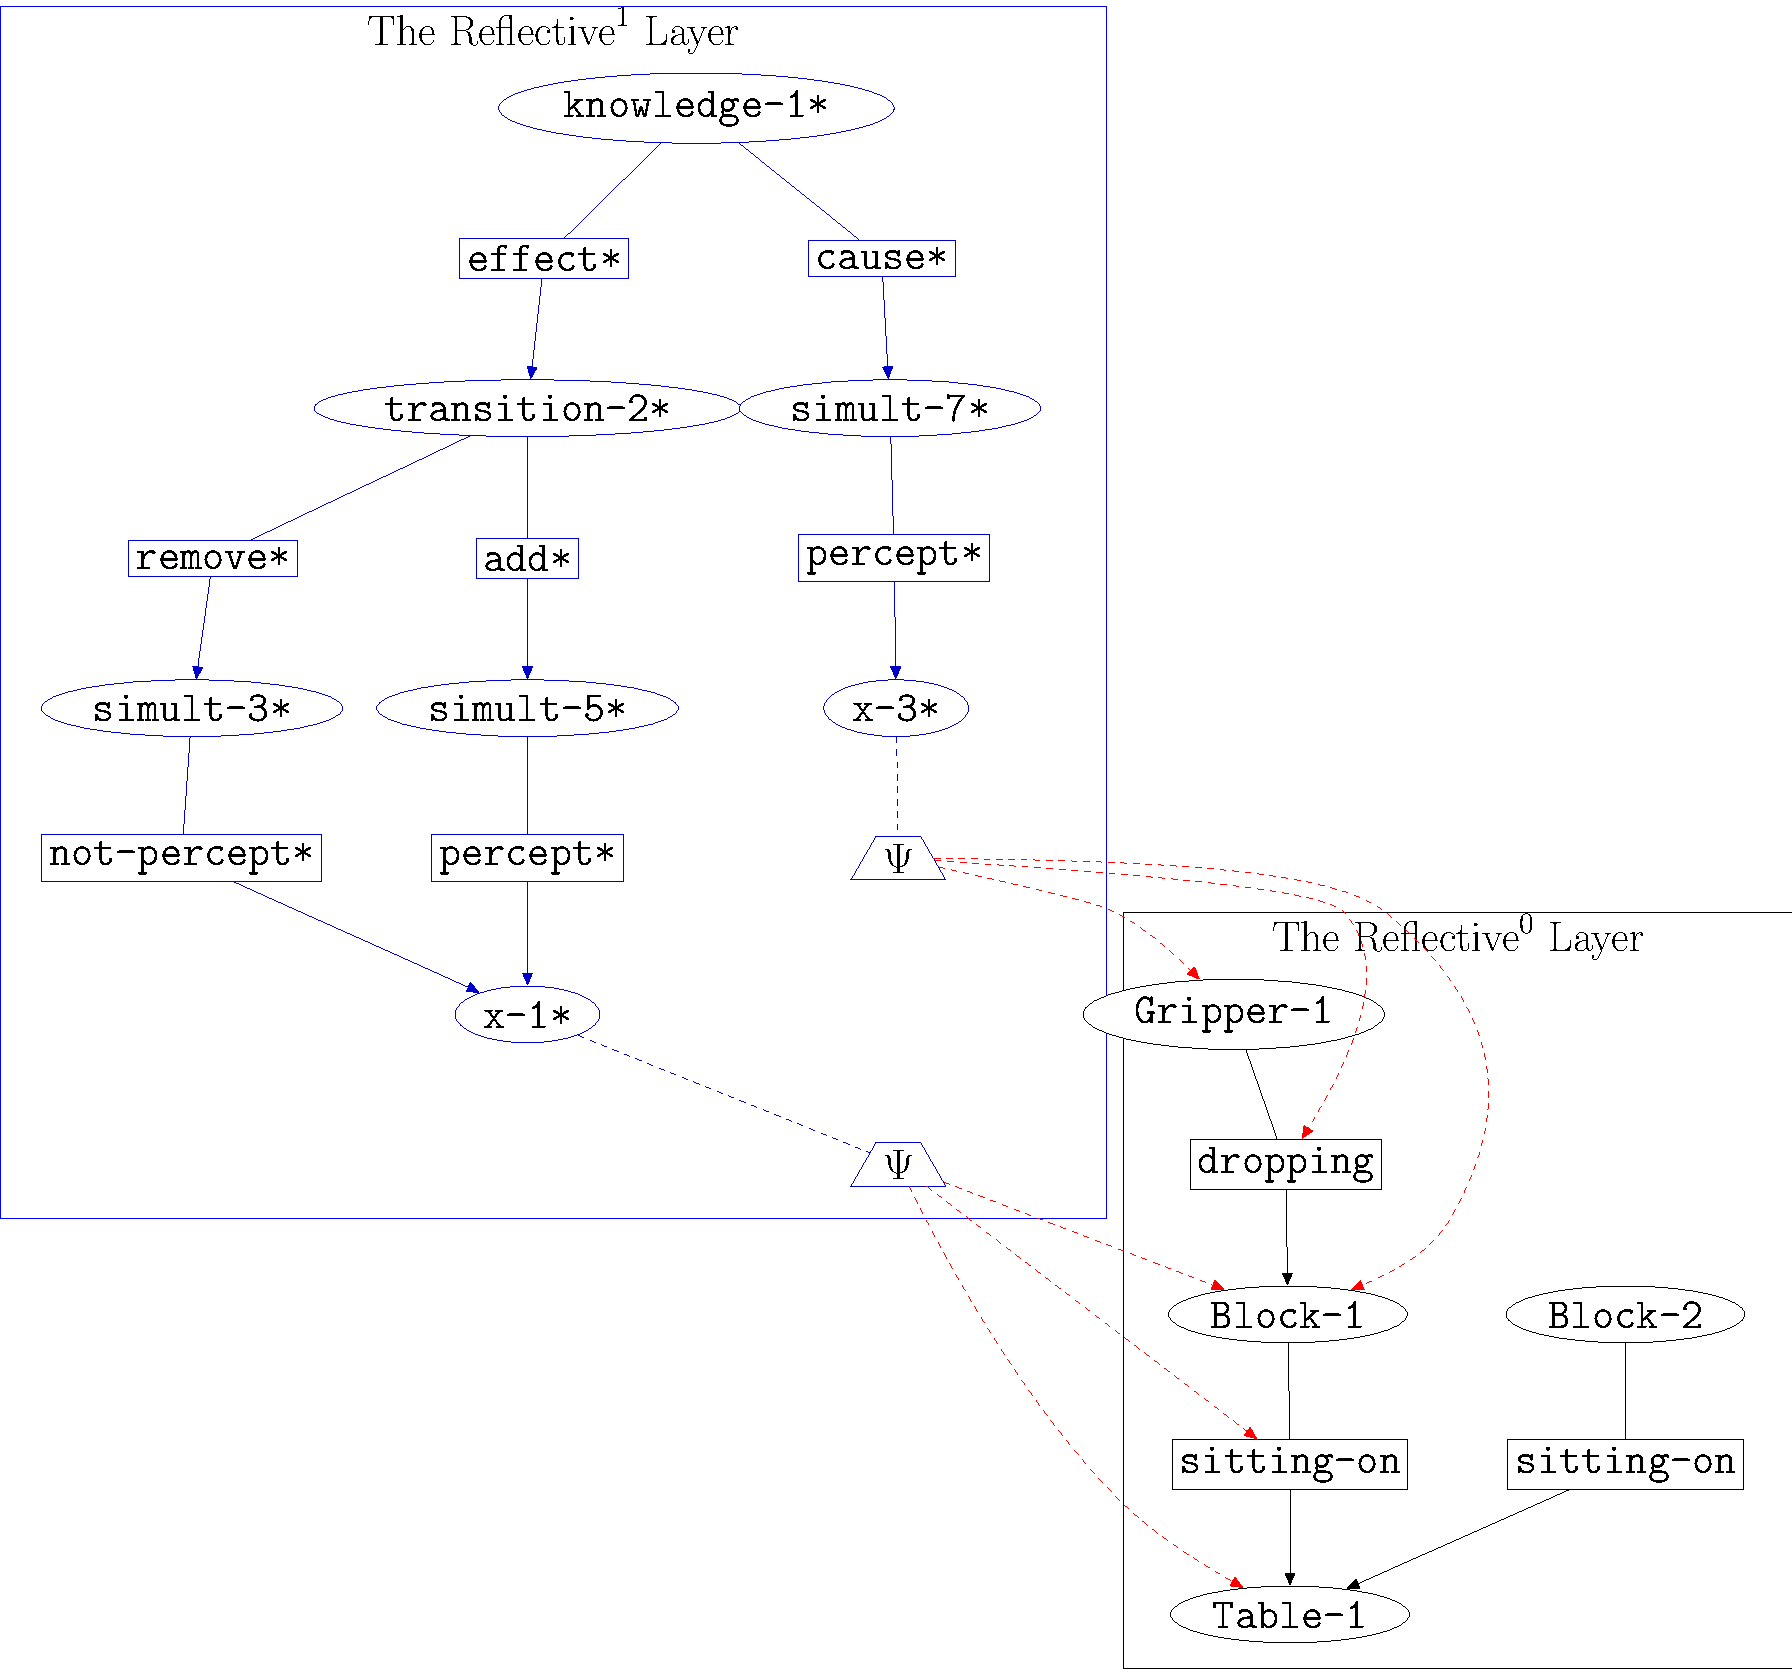
\includegraphics[width=12cm]{gfx/example_causal_knowledge}
\caption[An example of a causal knowledge.]{An example of causal
  knowledge, $\text{\tt{knowledge}}_1^*$, where the simultaneity,
  $\text{\tt{simult}}_7^*$, is known to be the cause of the
  transframe, $\text{\tt{transition}}_2^*$.  Negative perceptions are
  omitted here for to reduce visual clutter.}
\label{figure:example_causal_knowledge}
\end{figure}

\section{Representing Causal Hypotheses}

{\mbox{\autoref{figure:example_causal_hypothesis}}} shows an example
of a causal hypothesis, $h_1^*$, where the simultaneity,
$\text{\tt{simult}}_7^*$, is hypothesized to be the cause of the
transframe, $\text{\tt{transframe}}_2^*$.  In other words, the gripper
dropping the block causes the block to be sitting on the table.
\begin{figure}
\center
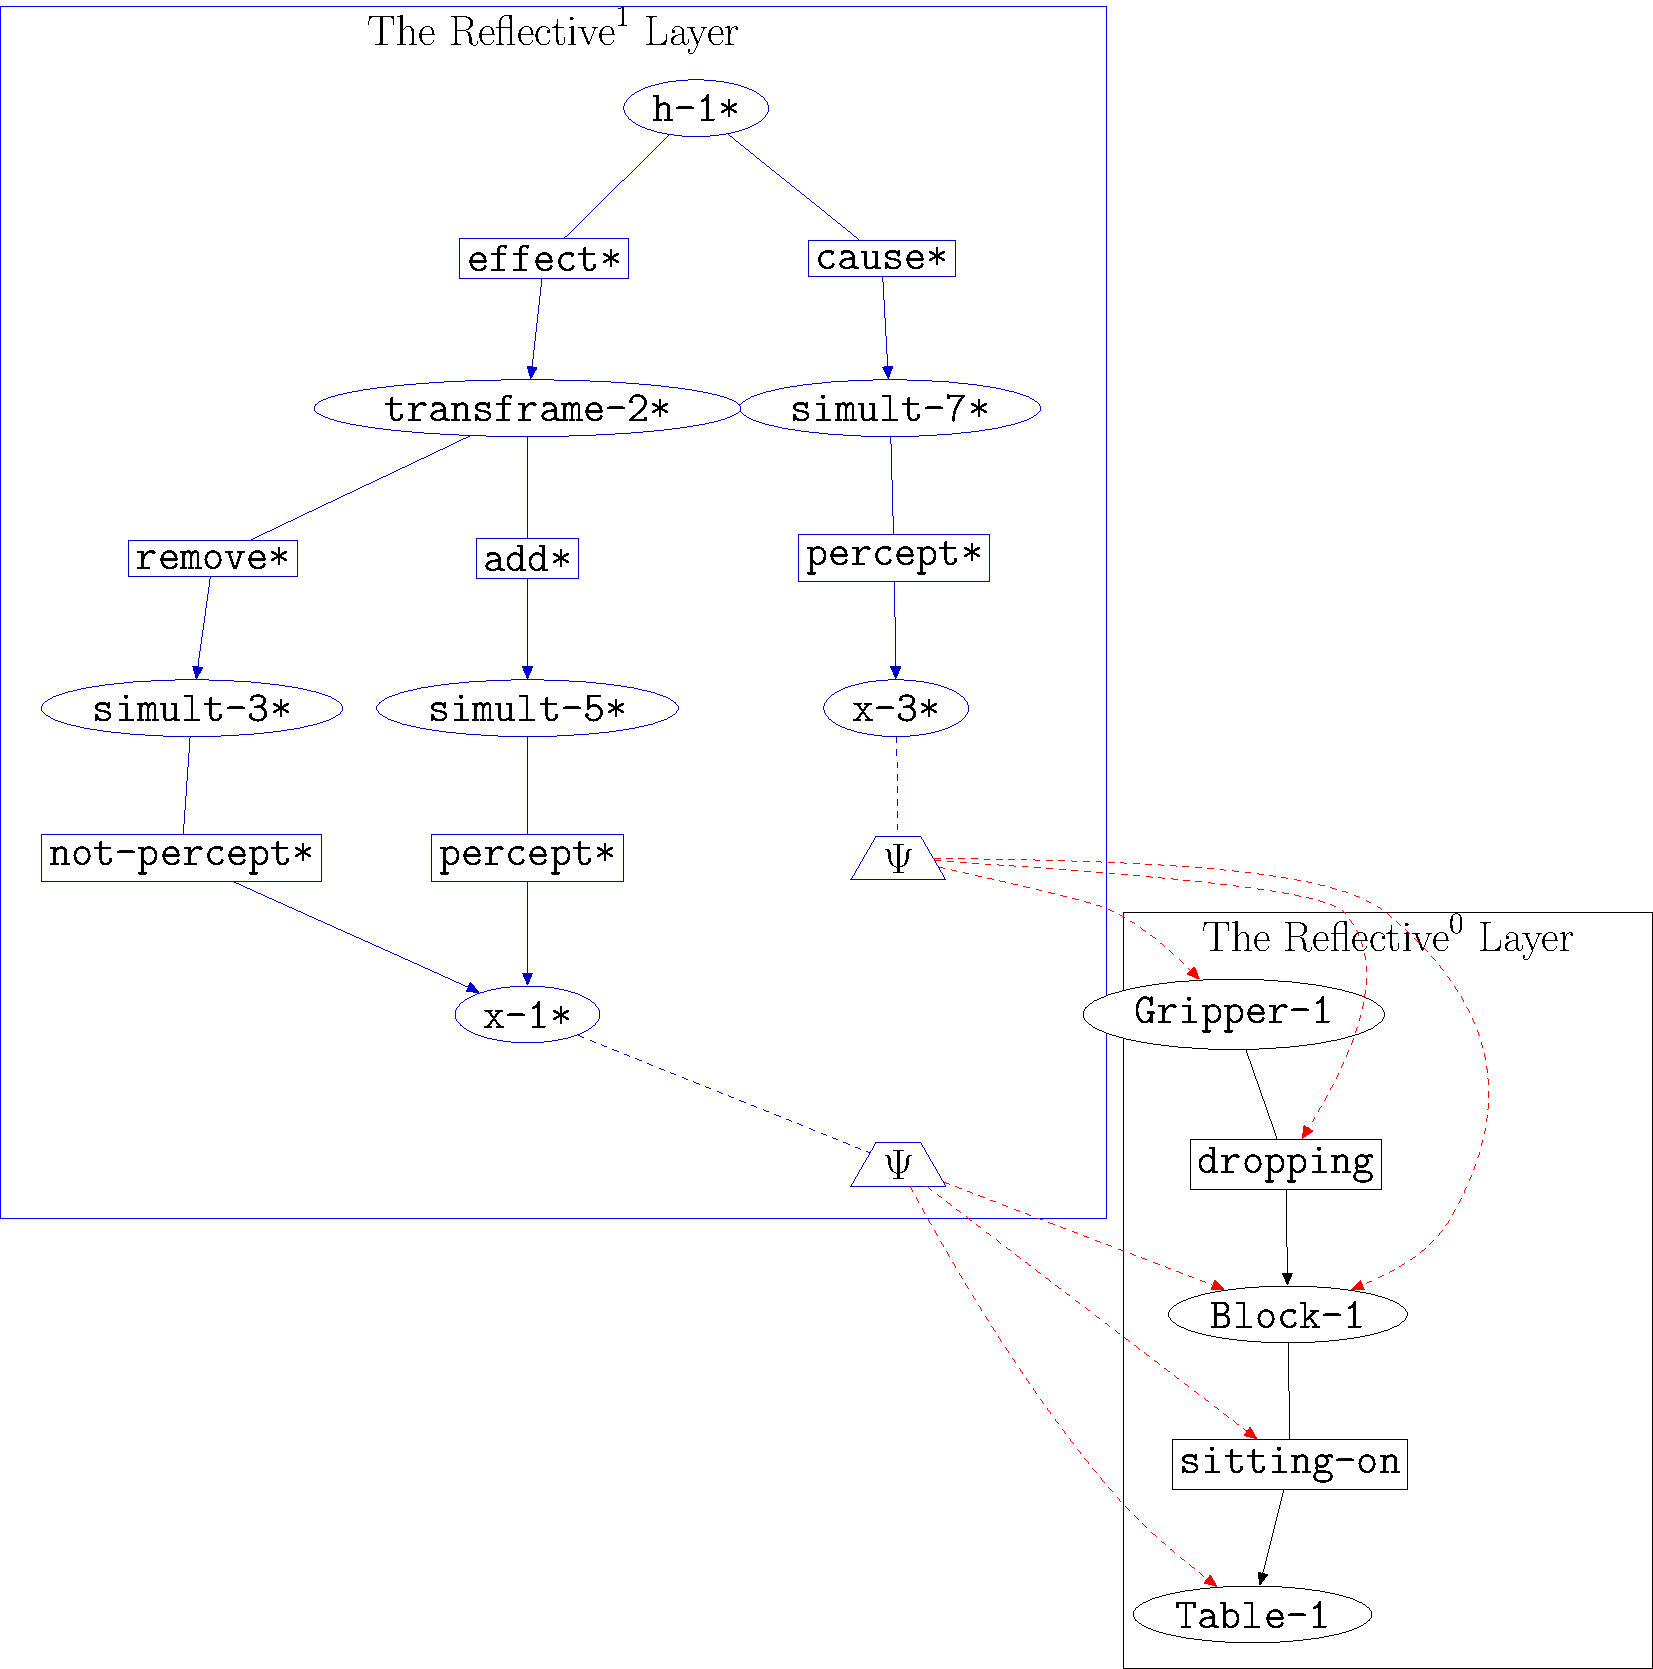
\includegraphics[width=8cm]{gfx/example_causal_hypothesis}
\caption[An example of a causal hypothesis.]{An example of a causal
  hypothesis, $h_1^*$, where the simultaneity,
  $\text{\tt{simult}}_7^*$, is hypothesized to be the cause of the
  transframe, $\text{\tt{transframe}}_2^*$.  In other words, the
  gripper dropping the block causes the block to be sitting on the
  table.}
\label{figure:example_causal_hypothesis}
\end{figure}

\section{Composing Plans from Hypotheses}

